% Created 2025-10-09 tor 10:12
% Intended LaTeX compiler: pdflatex
\documentclass[a4paper, 12pt]{article}
\usepackage[utf8]{inputenc}
\usepackage[T1]{fontenc}
\usepackage{graphicx}
\usepackage{longtable}
\usepackage{wrapfig}
\usepackage{rotating}
\usepackage[normalem]{ulem}
\usepackage{amsmath}
\usepackage{amssymb}
\usepackage{capt-of}
\usepackage{hyperref}
\usepackage[danish]{babel}
\usepackage[margin=3.0cm]{geometry}
\usepackage{hyperref}
\hypersetup{colorlinks, linkcolor=black, urlcolor=blue}
\setlength{\parindent}{0em}
\parskip 1.5ex
\author{Jacob Debel}
\date{Fysik A (Fysik B)}
\title{Opgaver til impuls og stød\\\medskip
\large Translatorisk mekanik}
\hypersetup{
 pdfauthor={Jacob Debel},
 pdftitle={Opgaver til impuls og stød},
 pdfkeywords={},
 pdfsubject={},
 pdfcreator={Emacs 30.2 (Org mode 9.7.11)}, 
 pdflang={Danish}}
\begin{document}

\maketitle
\section*{Opgave 1}
\label{sec:orga786a53}
En kraft på 50 N påvirker et objekt på 20 kg i 4 s. Derved standses objektet.

\begin{enumerate}
\item Bestem objektets impulsændring.
\item Bestem objektets oprindelige hastighed.
\end{enumerate}
\section*{Opgave 2}
\label{sec:orgc5af8ba}


\begin{wrapfigure}{r}{7cm}
\centering
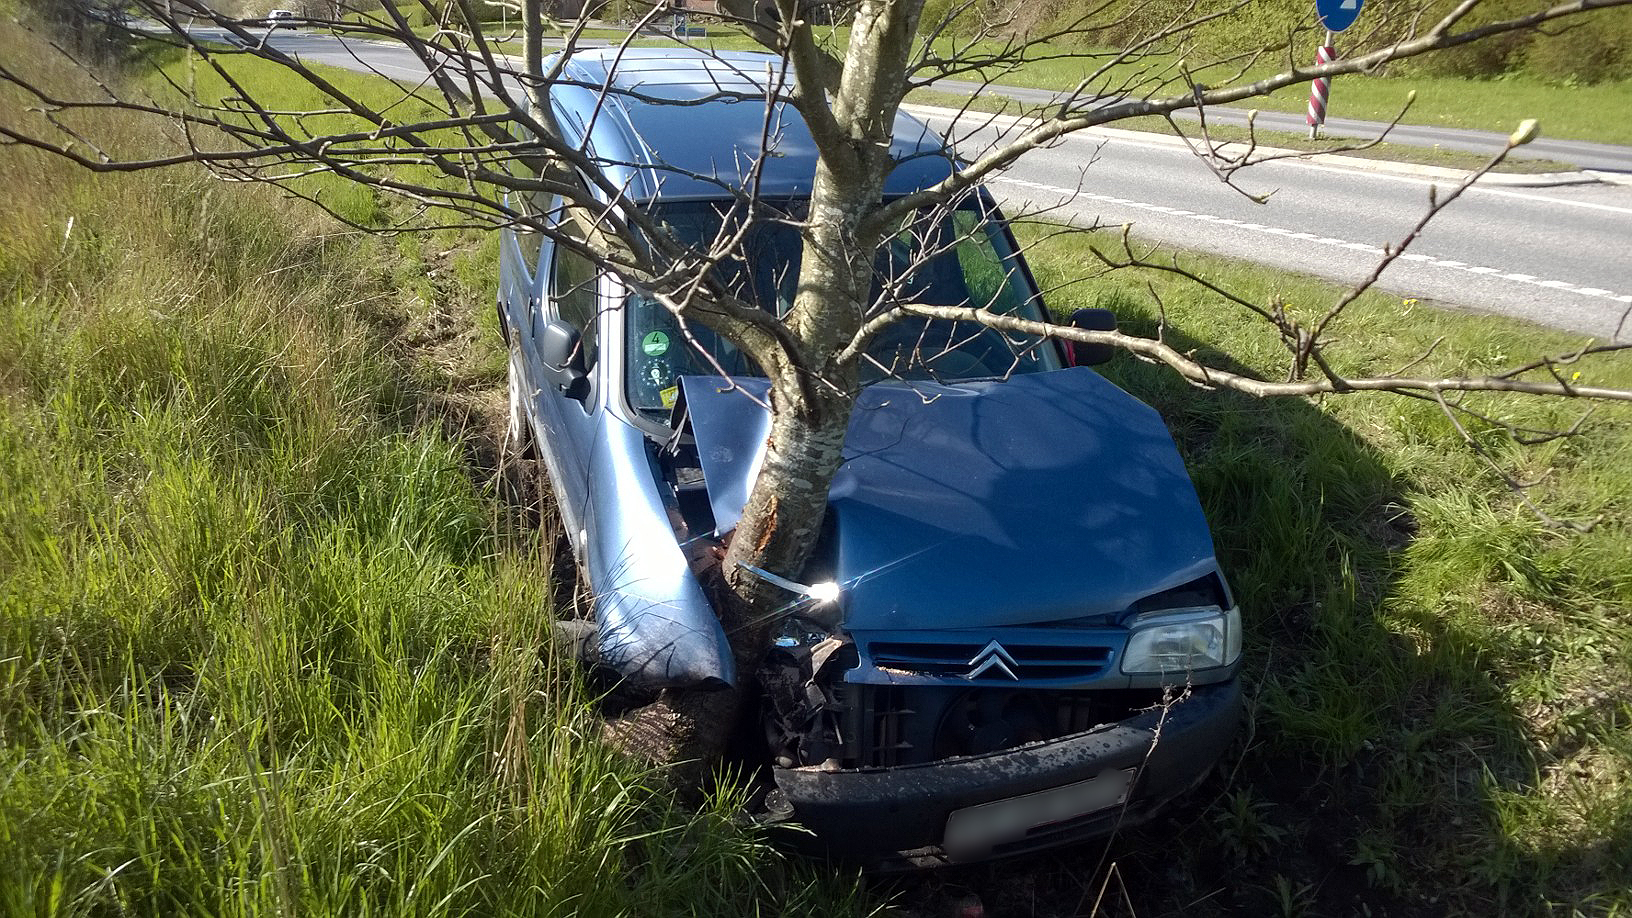
\includegraphics[width=7cm]{img/2019-12-16_08-51-29_WP_20150503_004.jpg}
\end{wrapfigure}

En 850 kg tung bil støder ind i et vejtræ med en hastighed på 40 km/h. Ved sammenstødet, som tager 0.15 s, deformeres bilens stødzone foran.

\begin{enumerate}
\item Bestem gennemsnitskraften på bilen.
\item Bestem gennemsnitsaccelerationen.
\item Bestem bilens deformation.
\end{enumerate}

\newpage
\section*{Opgave 3}
\label{sec:org64bb5ff}

\begin{center}
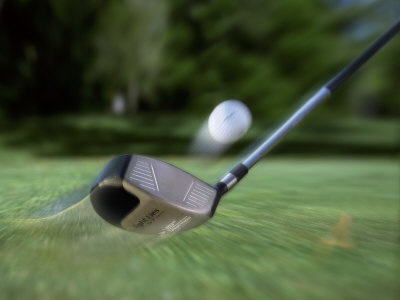
\includegraphics[width=7cm]{img/2019-12-16_08-54-03_7418334_orig.jpg}
\end{center}

En golfkugle opnår hastigheden 100 km/h ved et slag, som tager 2/100 s.
\begin{enumerate}
\item Bestem kraftpåvirkningen af den 150 g tunge golfkugle.
\end{enumerate}
\section*{Opgave 4}
\label{sec:orgb31953c}

\begin{center}

\includegraphics[width=10cm]{img/2019-12-16_08-55-46_slaa-soem-i.jpg}
\end{center}

Med et hammerslag bankes et søm ind i et stykke træ. Hammerens hoved vejer 500 g, og anslaget sker med en hastighed på 3.8 m/s, og tager 3/100 s.

\begin{enumerate}
\item Bestem impulsændringen af hammerhovedet.
\item Bestem den kraft hammeren påvirker sømmet med.
\item Bestem hvor langt sømmet slås ind.
\end{enumerate}
\section*{Opgave 5}
\label{sec:org677d5e6}
\begin{center}
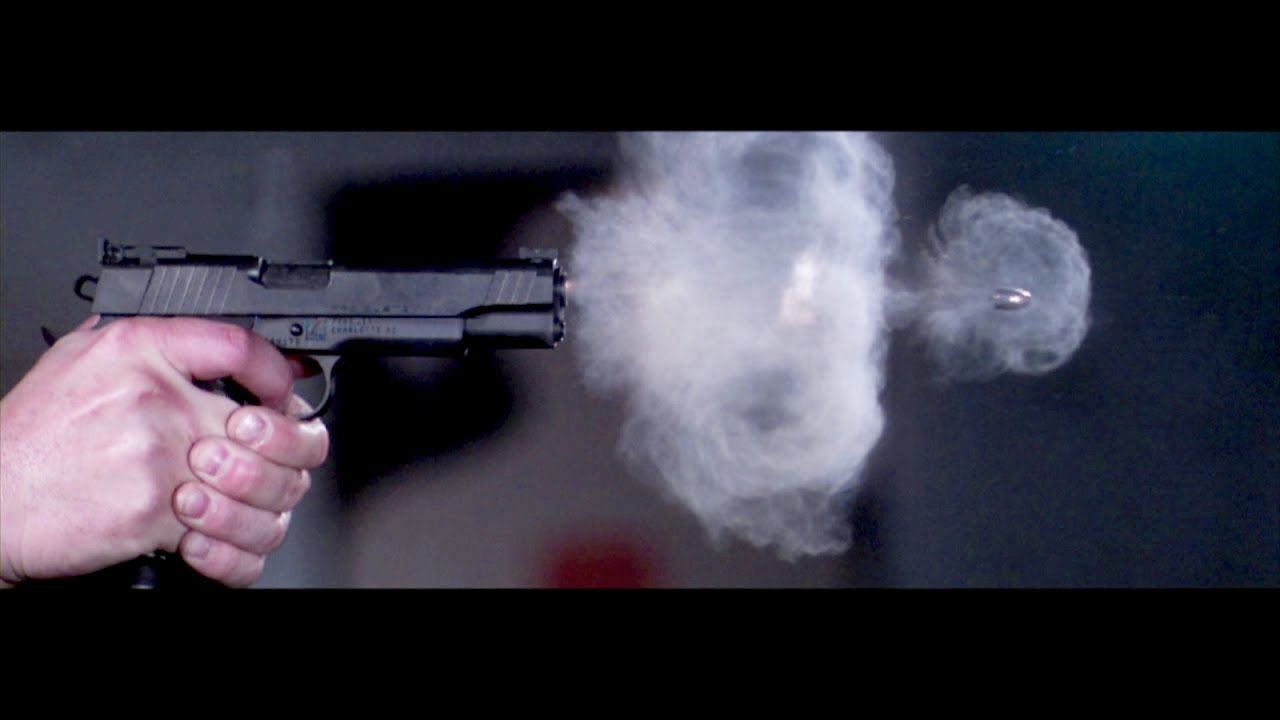
\includegraphics[width=10cm]{img/2019-12-16_08-58-54_an-incredible-super-slow-motion.jpg}
\end{center}

Et projektil på 20 g affyres af en pistol, som vejer 0.87 kg. Pistolløbet er 10 cm langt, og mundingshastigheden er 600 m/s. Pistolen holdes fast under skuddet.

\begin{enumerate}
\item Bestem pistolens rekylhastighed.
\item Bestem projektilets gennemsnitsacceleration.
\item Bestem rekylkraften, altså kraftpåvirkningen på pistolen.
\item Bestem gennemsnitskraften på pistolen taget over 1/10 s.
\end{enumerate}
\section*{Opgave 6}
\label{sec:org761502e}
\begin{center}
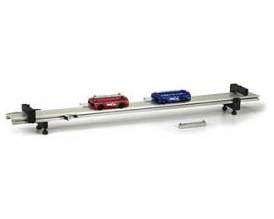
\includegraphics[width=7cm]{img/2019-12-16_09-00-56_20119914190724749.jpg}
\end{center}

En vogn med massen 300 g er i hvile, og en anden vogn med massen 430 g støder totalt uelastisk ind i denne. Vognen i bevægelse har hastigheden 2.73 m/s.

\begin{enumerate}
\item Bestem hastigheden efter stødet.
\item Bestem hastighederne af hver vogn efter stødet, hvis dette havde været 100\% elastisk.
\end{enumerate}

\newpage
\section*{Opgave 7}
\label{sec:org72a0cdb}
En af de store farer for Jorden er kometer og meteorer. Eksempelvis kan en komet med en masse på \(50 \cdot 10^9\) kg risikere at ramme Jorden med en hastighed på 40 km/s relativt til Jorden.

\begin{enumerate}
\item Bestem hastigheden af Jorden efter stødet i forhold til Jordens bane umiddelbart før stødet.
\item Bestem tabet i mekanisk energi.
\item Bestem hvor mange atombomber meteornedslaget svarer til. Antag af hver atombombe har en springkraft på 10 Megaton (\(5.066 \cdot 10^{16} J\)).
\end{enumerate}
\section*{Opgave 8}
\label{sec:orga444aa4}
\begin{center}
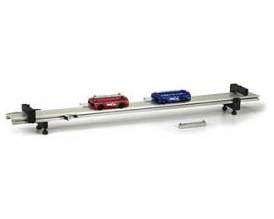
\includegraphics[width=7cm]{img/2019-12-16_09-00-56_20119914190724749.jpg}
\end{center}
To vogne med masser på henholdsvis 240 g og 462 g bevæger sig mod hinanden med hastigheder på henholdsvis 3.40 m/s og 4.28 m/s.

\begin{enumerate}
\item Bestem hastigheden efter stødet, såfremt dette er totalt uelastisk.
\item Bestem hastighederne efter stødet, såfremt dette havde været 100\% elastisk.
\end{enumerate}
\section*{Opgave 9}
\label{sec:org46e170f}
\begin{center}
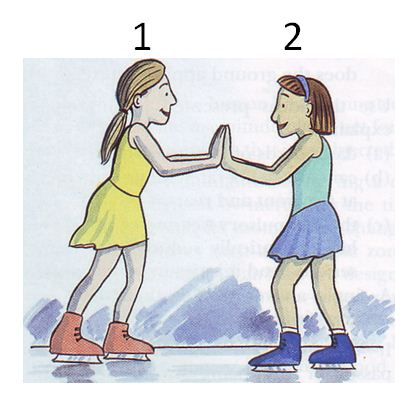
\includegraphics[width=7cm]{img/2019-12-16_09-03-52_forces+in+pairs.JPG}
\end{center}
To skøjteløbere, der tilsammen vejer 120 kg, står over for hinanden, og puffer til hinanden, så de bevæger sig fra hinanden med hastigheder på 3.3 m/s og 2.1 m/s.
\begin{enumerate}
\item Bestem de to skøjteløberes individuelle vægte.
\end{enumerate}
\section*{Opgave 10}
\label{sec:org4eeebb0}
En træklods med massen 0.85 kg ligger i hvile på et vandret underlag, hvor friktionskoefficienten er \(\mu = 0.25\). Et projektil, med massen 5 g skydes ind i træklodsen vandret, hvor det sætter sig fast. Træklodsen bevæger sig herefter 2.0 m, før den går i stå igen.
\begin{enumerate}
\item Bestem klodsens hastighed, lige efter projektilet har boret sig fast.
\item Bestem projektilets hastighed umiddelbart før det rammer træklodsen.
\item Bestem tabet i mekanisk energi i procent fra før projektilet rammer klodsen, til lige i det øjeblik, hvor projektilet har sat sig fast i klodsen.
\end{enumerate}

\newpage
\section*{Opgave 11}
\label{sec:org0f202c2}
\begin{center}
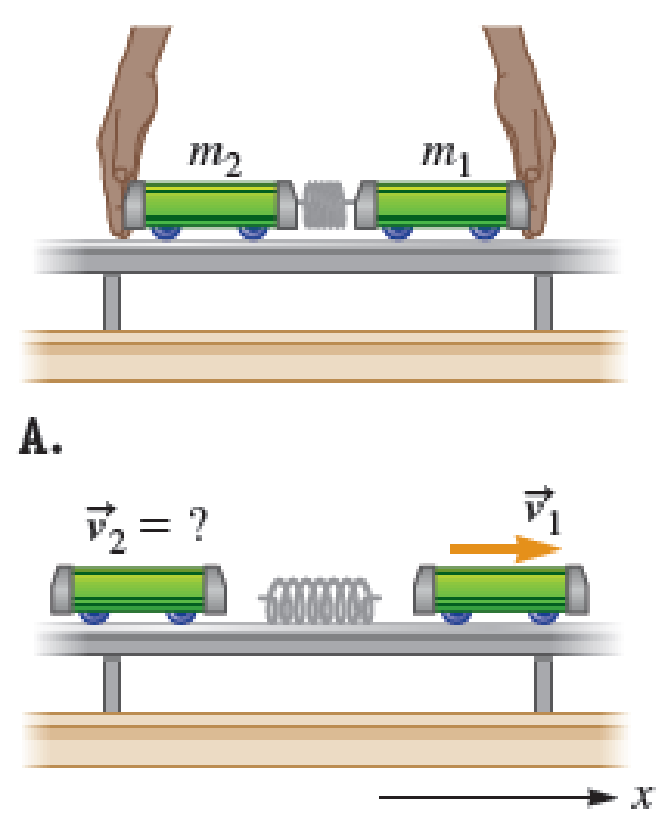
\includegraphics[width=7cm]{img/2019-12-16_09-08-12_39146-10-40pq-question-digital_image_001.png}
\end{center}

En fjeder med fjederkonstanten 650 N/m presses ind mellem to vogne, således at dens deformation er 4.2 cm. Vognenes masser er henholdsvis 2.7 kg og 4.82 kg.
\begin{enumerate}
\item Bestem hastighederne efter at fjederen er udløst.
\end{enumerate}
\section*{Opgave 12}
\label{sec:org4f90533}
Et projektil på 17 g skydes ind i en 3.96 kg tung sandsæk. Sandsækken er ophængt i en 2 m lang snor, og gør ved skuddet et udsving på \(37^{\circ}\) med lodret.

\begin{enumerate}
\item Bestem hastigheden af sandsækken umiddelbart efter at projektilet har sat sig fast.
\item Bestem projektilets hastighed umiddelbart før det ramte sandsækken.
\end{enumerate}
\section*{Opgave 13}
\label{sec:orgd9f4112}
En satellit på ialt 500 kg er udstyret med en brændstoftank på 50 kg. Ved forbrænding af brændstoffet slynges dette bagud gennem dyser med en hastighed på 4500 m/s.
\begin{enumerate}
\item Beregn den hastighedsændring, som brændstoffet kan give satellitten, når denne befinder sig i det fri rum.
\end{enumerate}
\section*{Opgave 14}
\label{sec:orge8261bb}
En 70 kg tung kugle med en diameter på 50 cm forbindes til enden af en 30 kg tung homogen bjælke med med en længde på 1.3 m.

\begin{enumerate}
\item Indlæg et passende koordinatsystem og angiv massemidtpunkterne af kuglen og bjælken.
\item Bestem beliggenheden af systemets massemidtpunkt.
\end{enumerate}
\section*{Opgave 15}
\label{sec:org55c26d6}
Tre stænger med ensartert tværsnit og massefylde svejses sammen til en trekant med sidelængder 1.5 m, 2 m og 2.5 m.
\begin{enumerate}
\item Beregn beliggenheden af trekantens massemidtpunkt.
\end{enumerate}
\section*{Facitliste}
\label{sec:org2a1dc22}

\begin{itemize}
\item \textbf{Opgave 1:} 1) 200 Ns 2) 10 m/s
\item \textbf{Opgave 2:} 1) 62.96 kN 2) \(74 m/s^2\) 3) 0.83 m
\item \textbf{Opgave 3:} 1) 208 N
\item \textbf{Opgave 4:} 1) \(1.9 \frac{kg \cdot m}{s}\) 2) 63.3 N 3) 5.7 cm
\item \textbf{Opgave 5:} 1) 13.8 m/s 2) \(1.8 \cdot 10^6 m/s^2\) 3) 36 kN 4) 120 N
\item \textbf{Opgave 6:} 1) 1.61 m/s 2) 3.22 m/s og 0.486 m/s
\item \textbf{Opgave 7:} 1) 0.335 nm/s 2) \(4.0\cdot 10^{19} J\) 3) 790
\item \textbf{Opgave 8:} 1) -1.65 m/s 2)-6.78 m/s og 1.01 m/s
\item \textbf{Opgave 9:} 1) 73.3 kg og 46.7 kg
\item \textbf{Opgave 10:} 1) 3.13 m/s 2) 533 m/s 3) 99.4\%
\item \textbf{Opgave 11:} 1) -0.52 m/s og 0.29 m/s
\item \textbf{Opgave 12:} 1) 2.81 m/s 2) 654 m/s
\item \textbf{Opgave 13:} 1) 474 m/s
\item \textbf{Opgave 14:} 1) ikke noget facit 2) 0.27 m fra kuglens centrum.
\item \textbf{Opgave 15:} 1) x= 0.75 m og y=0.5 m (afhænger af placeringen af stængerne i koordinatsystemet).
\end{itemize}
\end{document}
